Si vuole realizzare mediante Arduino un circuito che stimi la concentrazione dell’alcool e in base al valore letto dal sensore \textit{MQ-3} regoli l’accensione delle luci di una LED bar. Sono stati utilizzati i seguenti componenti:
\begin{itemize}
    \item Resistenze $R_1$, $R_2$, $R_0=\dots=R_n$ da determinare, 0.25 W.
    \item LED bar,  codice \textit{DC10SRWA}, Kingbright 
    \item Sensore alcool \textit{MQ-3}
    \item Scheda Arduino DUE
\end{itemize}
Il circuito riportato in Figura \ref{fig:CircuitFacAlcool} è alimentato mediante porta USB del PC, la quale eroga circa $(\sim 5 V)$
\begin{figure}[H]
    \centering
    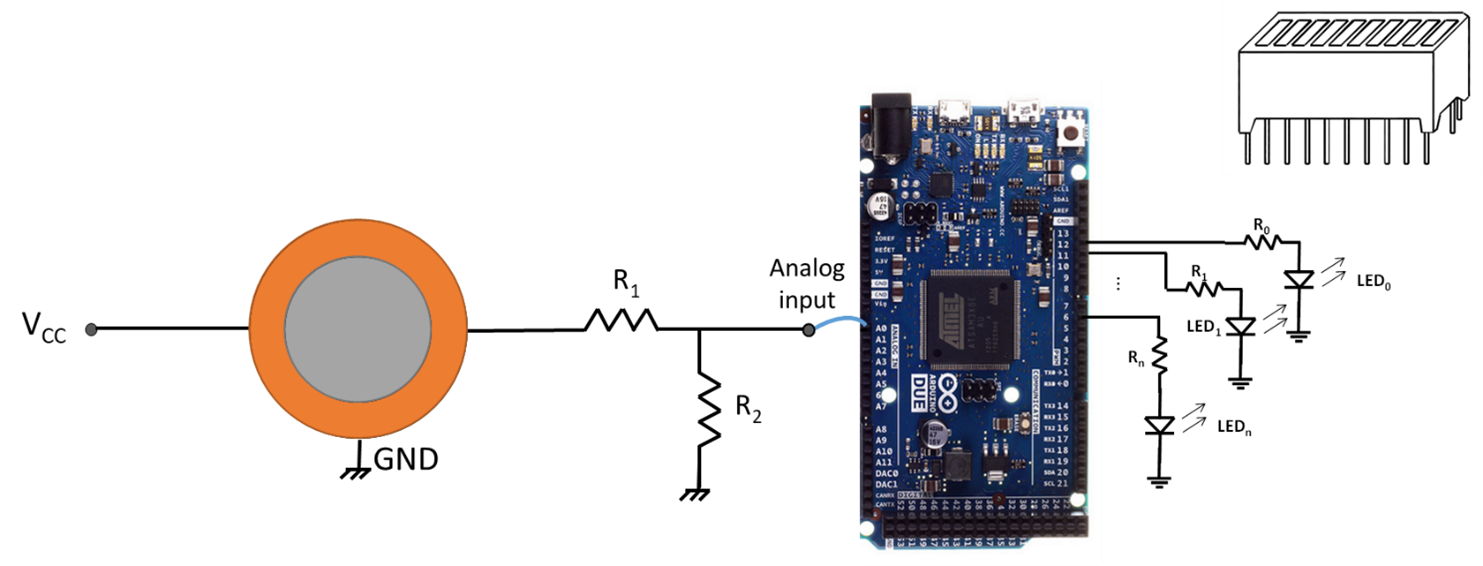
\includegraphics[width=0.7\linewidth]{images/CircuitFacAlcool.png}
    \caption{Schema circuito}
    \label{fig:CircuitFacAlcool}
\end{figure}
I vari LED della LED bar a 10 segmenti sono collegati ai pin digitali \textbf{12\dots3} mentre il sensore \textit{MQ-3} è collegato al pin analogico \textbf{A0} tramite il partitore di tensione $R_1$ e $R_2$.
\subsection{In laboratorio}
Le resistenze $R_1$ e $R_2$ sono state dimensionate in modo da ottenere:
\begin{itemize}
    \item Tensione in ingresso all’Arduino pari a $3.3\text{ V}$ 
    \item Una resistenza totale di $200\text{ k}\Omega$
\end{itemize}
Il sensore \textit{MQ-3} viene alimentato dalla tensione di 5 V. Abbiamo alimentato il sensore e misurato la tensione di uscita del sensore, che risulta essere 4.64 V. Volendo ottenere ai capi di $R_2$ la tensione di 3.3 V abbiamo dimensionato il partitore di tensione come segue:
\begin{equation}
    \begin{cases}
        R_1+R_2=200\text{ k}\Omega\\
        4.64\text{V}\cdot\frac{R_2}{R_1+R_2}=3.3\text{ V}
    \end{cases}
    \implies R_1=58\text{ k}\Omega\quad R_2=142\text{ k}\Omega
\end{equation}
Quindi sono state utilizzate le resistenze
\begin{equation*}
    R_1 = 56 \text{ k} \Omega\quad R_2 = 150 \text{ k} \Omega
\end{equation*}
Successivamente, sono state dimensionate le resistenze $R_0=\dots=R_n$, sapendo che la massima corrente erogata dai pin digitali è $3\text{ mA}$. Sapendo che i LED del display hanno tensione operativa pari a $V_{ON}=2.3\text{ V}$ abbiamo scelto le resistenze
\begin{equation*}
    R_i=\frac{V_{CC}-V_{ON}}{3\text{ mA}}=333.33\Omega\implies R_0=\dots=R_n = 470\Omega
\end{equation*}
\subsection{Codice}
Infine si è scritto il codice necessario per realizzare l’etilometro. Si vuole che le luci della LED bar si accendano in accordo al valore letto dal sensore. L’obiettivo è di avere 10 luci accese quando la concentrazione è massima e 1 luce accesa quando la concentrazione è minima.
\begin{lstlisting}[frame=single, language=Arduino]
const int alcolPin = A0;
const int matrixPin[10] = {12,11,10,9,8,7,6,5,4,3};

void setup(){
    for(int i = 0; i < 10; i++){
        pinMode(matrixPin[i], OUTPUT);
        digitalWrite(matrixPin[i], LOW);
    }
}

void loop(){
    int alcolValue = analogRead(alcolPin);
    int alcolValue2 = map(alcolValue, 940, 990, 0, 9);
    for(int i = 0; i < 10; i++){
        if(i < alcolValue2){
            digitalWrite(matrixPin[i], HIGH);
        }else{
            digitalWrite(matrixPin[i], LOW);
        }
    }
}
\end{lstlisting}
Abbiamo verificato il corretto funzionamento del programma avvicinando un batuffolo di cotone imbevuto di alcool al sensore e osservando la reazione del circuito sulla LED bar.